\documentclass[12pt]{report}
\usepackage[utf8]{inputenc}
\usepackage[italian]{babel}
\usepackage{amsmath}
\usepackage{graphicx}
\title{Tecniche automatiche per dimostrare la segretezza forte nei protocolli crittografici}
\author{Gianluca Lutero}

\begin{document}
\maketitle
\newpage
%\tableofcontents

\newpage
\addcontentsline{toc}{section}{Introduzione}
\section*{Introduzione}
\section*{Calcolo dei processi}
% Descrivere brevemente sintassi e semantica del calcolo dei processi
Per rappresentare i protocolli viene utilizzato il formalismo del calcolo dei processi con l'aggiunta delle primitive crittografiche probabilistiche. Di seguito viene mostrata la sintassi:\\
\begin{figure}[h]
    \centering
    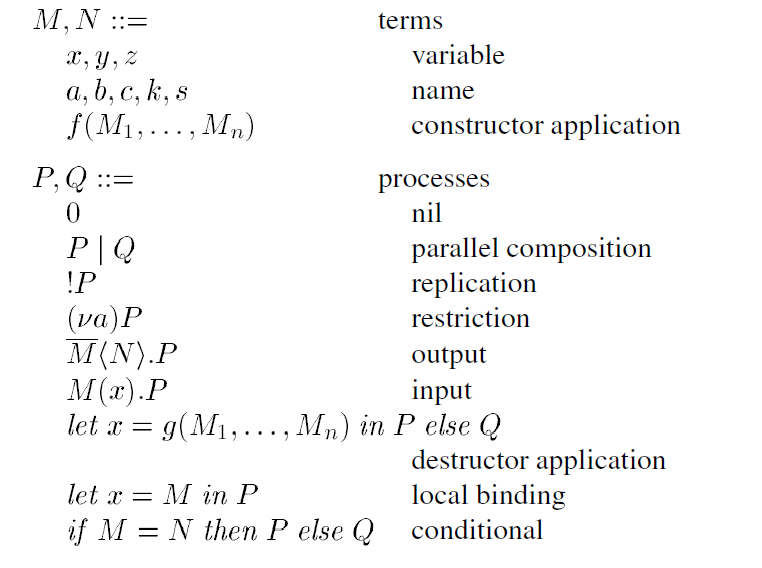
\includegraphics[scale=0.5]{Relazione/Immagini/calcolo.PNG}
\end{figure}\\
Si assumono un infinito numero di nomi e variabili e un insieme di simboli per i costruttori e i distruttori. Per convenzione vengono usate le lettere $a, b, c, k$ per i nomi, $x, y, z$ per le variabili, $f$ per il costruttore e $g$ per il distruttore. Si definiscono termini le variabili, i nomi e le applicazioni di costruttore. Un distruttore è una funzione parziale che un processo può utilizzare per manipolare termini. Il formalismo include i costrutti standard del $\pi$-calcolo.\\
L'uso dei costruttori e dei distruttori permette di rappresentare strutture dati e operazioni crittografiche. Vengono definiti inoltre le funzioni $fn(P)$ e $fv(P)$ che restituiscono rispettivamente i nomi e le variabili libere nel processo P. Un processo si dice chiuso se non ha variabili libere. La semantica del formalismo è definita dalla relazione di riduzione $ \xrightarrow{} $ e dalla relazione di equivalenza strutturale $ \equiv$.
\section*{Segretezza forte}
% Definizioni
Per formalizzare il concetto di segretezza forte si passa dalla seguente definizione di equivalenza osservazionale:\\

\textbf{Definizione:}  Un contesto di valutazione $C$ é un contesto costruito a partire da $[], C | P, P|C \hspace{2mm}e\hspace{2mm} (\nu a)C.$\\
$P$ emette su $m$, $P \Downarrow m$, se e solo se $P (\leftarrow \cup \equiv)* C[\overline{m}\langle N \rangle.R]$ dove $C$ é un contesto di valutazione che non lega $m$.\\

Si definisce equivalenza osservazionale $\approx$ la piú grande relazione simmetrica $R$ tra processi chiusi tale che $PRQ$ implica:\\
\begin{enumerate}
    \item se $P \Downarrow m$ allora $Q \Downarrow m$
    \item se $P \leftarrow P'$ allora esiste $Q$ tale che $Q \leftarrow^* Q'$ e $P'RQ'$
    \item $C[P]RC[Q]$ per tutti i contesti di valutazione chiusi $C$.
\end{enumerate}
Un processo $P$ emette su $m$ quando, dopo un qualsiasi numero di passi di riduzione, questi manda un messaggio su $m$ e l'avversario ottiene $m$. In questo modo l'output del canale $m$ é osservabile dall'avversario. Questo fatto é sfruttato nel punto 1 della definizione: per $P$ e $Q$ equivalenti osservazionalmente, se $P$ emette su $m$ allora anche $Q$ emette su $m$, se così non fosse l'avversario sarebbe in grado di distinguerli. Nel punto 2 viene mostrato che la proprietà é preservata dalla riduzione. Questo punto fa sì che la struttura della riduzione sia visibile all'avversario: quando $P$ e $Q$ sono osservazionalmente equivalenti, se $P$ si riduce in modo non deterministico in due processi non equivalenti $P'$ e $P''$, allora anche $Q$ si riduce in due processi $Q'$ e $Q''$ osservazionalmente equivalenti rispettivamente a $P'$ e $P''$. Il punto 3 prende in considerazione l'avversario, rappresentato da un qualsiasi contesto chiuso di valutazione, ossia un contesto di valutazione tale che $C[P]$ e $C[Q]$ sono chiusi. A questo punto può essere data la definizione di segretezza forte attraverso il concetto per cui l'avversario non può distinguere due processi che differiscono per il valore dei messaggi cifrati.\\

\textbf{Definizione:} Il processo $P_0$ preserva la segretezza forte delle sue variabili libere se e solo se per ogni sostituzione chiusa $\sigma$ e $\sigma'$ di dominio $fv(P_0)$ , $\sigma P_0 \approx \sigma' P_0$.\\

Intuitivamente se il processo ha una falla allora esiste un contesto $C$ che può sfruttarla per eseguire differenti output a seconda del valore del messaggio scambiato, per cui $C[\sigma P_0]$ e $C[\sigma' P_0]$ non soddisfano il punto 1 della definizione di equivalenza osservazionale. Viene dato adesso un criterio più forte per dimostrare la segretezza forte. Intuitivamente viene richiesto che per ogni passo di riduzione questa proceda in modo uniforme per tutti i valori dei termini. Per un passo di comunicazione questo significa che il canale deve essere pubblico. Per un distruttore questo significa che il successo o il fallimento del processo indipendentemente dal valori dei messaggi.\\

\textbf{Proposizione 1:} Sia $Secr$ l'insieme dei nomi che contiene tanti elementi quanti sono $fv(P_0)$  e tale che $fn(P_0) \cap Secr = \emptyset$. Sia $\sigma$ una sostituzione che mappa tutte le variabili libere di $P_0$ ad elementi distinti di $Secr$. Si assume allora che per tutti $Q$ tale che $fn(Q) \cap Secr = \emptyset$:
\begin{enumerate}
    \item se $\sigma P_0 | Q (\rightarrow \cup \equiv)^* C[\overline{M} \langle N \rangle . R]$ o $\sigma P_0 | Q (\rightarrow \cup \equiv)^* C[M(x).R]$ e $C$ è un contesto di valutazione tale che non leghi i nomi in $Secr$ allora $M \notin Secr$.
    
    \item se $\sigma P_0 | Q (\rightarrow \cup \equiv)^* C[let\ y\ =\ g(M_0,\dots,M_n)\ in\ Q'\ else\ R']$, $\theta$ è una sostituzione chiusa con $dom(\theta)\ =\ Secr$, $C$ è un contesto di valutazione che non lega nomi di $Secr$ o nelle immagini di $\theta$, $g(N_0,\dots,N_n) \rightarrow N$ è contenuta in $def(g)$, e $\theta (M_0,\dots,M_n)$ è un'istanza di $(N_0,\dots,N_n)$, allora anche $(M_0,\dots,M_n)$ è un'istanza di $(N_0,\dots,N_n)$   
\end{enumerate}
Allora $P_0$ preserva la proprietà di segretezza forte.\\

Il processo $Q$ rappresenta un qualsiasi avversario. Il secondo punto della proposizione indica che l'applicazione di un distruttore $g(M_0,\dots,M_n)$ ha successo per il valore dei messaggi dati da $\theta$ allora deve avere successo per qualsiasi valore del messaggio.\\ 

\textbf{Dimostrazione:} Per procedere devono prima essere riformulate le proposizioni precedenti usando il concetto di contesto per rappresentare l'avversario. Sia $C$ un contesto di valutazione. Sia $Secr'$ un insieme di nomi non libero o legati in $C$ e non liberi in $P_0$, contenenti tanti elementi quanti $fv(P_0)$. Sia $\sigma'_0$ una sostituzione che mappa le variabili libere di $P_0$ in $Secr'$.
\begin{enumerate}
    \item se $C[\sigma'_0 P_0] (\rightarrow \cup \equiv)^* C'[\overline{M} \langle N \rangle . R]$ o $C[\sigma'_0 P_0] (\rightarrow \cup \equiv)^* C'[M(x).R]]$ e $C'$ è un contesto di valutazione che non lega nomi in $Secr'$ allora $M \notin Secr'$.
    \item se $C[\sigma'_0 P_0] (\rightarrow \cup \equiv)^* C'[let\ y\ =\ g(M_0,\dots,M_n)\ in\ Q'\ else\ R']$, $\theta$ è una sostituzione chiusa con $dom(\theta)\ =\ Secr'$, $C'$ è un contesto di valutazione che non lega nomi di $Secr'$ o nelle immagini di $\theta$, $g(N_0,\dots,N_n) \rightarrow N$ è contenuta in $def(g)$, e $\theta (M_0,\dots,M_n)$ è un'istanza di $(N_0,\dots,N_n)$, allora anche $(M_0,\dots,M_n)$ è un'istanza di $(N_0,\dots,N_n)$ 
\end{enumerate}
Si definisce ora la relazione $R$ come $PRP'$ se e solo se esiste:\\
\begin{enumerate}
    \item un contesto di valutazione $C$
    \item un insieme $Secr'$ di nomi non liberi o legati in $C$ e non legati in $P_0$, contenenti tanti elementi quanti sono in $fv(P_0)$
    \item una sostituzione $\sigma'_0$ che mappa le variabili libere di $P_0$ ad elementi distinti di $Secr'$
    \item sostituzioni $\theta$ e $\theta'$ con dominio $Secr'$
    \item un processo chiuso $P''$ tale che $P\ =\ \theta P''$, $P'\ =\ \theta'P''$ e\\ $C[\sigma'_0 P_0]\ (\rightarrow \cup \equiv)^*\ P''$  
\end{enumerate}
La relazione $R$ è simmetrica. Si dimostra adesso che $R$ soddisfa i tre punti della definizione di equivalenza osservazionale.\\
\begin{itemize}
    \item La prova del punto 1 avviene usando l'ipotesi 1 mostrando che il canale non viene modificato da $\theta$ e $\theta'$
    \item La prova del punto 2 viene fatta per casi sulle riduzioni. Nel caso di una comunicazione viene usata l'ipotesi 1 per mostrare che il canale non viene modificato da $\theta$ e $\theta'$, in questo modo $ P\ =\ \theta P'',\ P'\ =\ \theta'P'' $ e $P''$ possono comunicare.Il caso dell'applicazione del distruttore usa l'ipotesi 2: se l'applicazione del distruttore ha successo in $P\ =\ \theta P''$ allora ha successo anche per $P''$ e $P'\ =\ \theta'P''$; se il distruttore fallisce in $P$ allora fallisce sia in $P''$ e $P'$ dato che se avesse avuto successo in $P'\ =\ \theta'P''$ per l'ipotesi 2 avrebbe implicato il successo anche in $P''$ e $P\ =\ \theta P''$
    \item La prova del punto 3 si basa sulla definizione di $R$. Il punto delicato della dimostrazione risiede nel rinominare i nomi in $Secr'$ per impedire la loro cattura dal contesto aggiunto
\end{itemize}
Allora $R \subset \ \approx$. In più per ogni sostituzione $\sigma$ e $\sigma'$ di dominio $fv(P_0)$ vale $\sigma P_0 R \sigma'P_0$, prendendo $C=[],\ Secr'\ =\ Secr,\ \sigma'\ =\ \sigma, \theta \ e\ \theta'$ tali che $\theta \sigma_0 \ =\ \sigma,\ e\ \theta'\sigma_0\ =\ \sigma', P'\ =\ \sigma_0 P_0$. In questo modo $P_0$ preserva la proprietà di segretezza forte delle sue variabili libere.

\section*{Primitive per la verifica del protocollo}
Adesso verrà esteso il formalismo del calcolo dei processi con le primitive per la verifica della proprietà di segretezza forte. Il sistema di verifica costruisce un insieme di clausole di Horn a partire da un processo chiuso $P_0$. Si assume che ogni restrizione $(\nu a)P$ in $P_0$ contiene un nome differente per $a$ e che quel nome sia differente per ogni nome libero in $P_0$. Si associa ad ogni replicazione in $P_0$ un identificare di sessione. Gli identificatori di sessione sono variabili che prendono valore da un insieme numerabile di termini e un valore diverso per ogni copia del processo replicato. Questo permette di distinguere le diverso copie del processo, in particolare vengono usati per distinguere i nomi generati dalle stesse restrizioni nelle differenti copie del processo. I termini delle regole sono chiamati pattern $p$ e sono generati dalla seguente grammatica:\\
\begin{figure}[h]
    \centering
    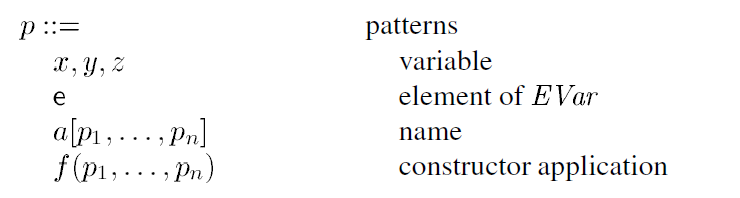
\includegraphics[scale=0.7]{Relazione/Immagini/rule.PNG}
\end{figure}\\
L'insieme $EVar$ contiene le costanti usate nel predicato $testunif$. Una restrizione in un processo crea sempre un nuovo nome ogni volta che questi viene eseguito. Quando una restrizione si trova all'interno di una replicazione, questo porta a generare un illimitato numero di nomi, il che porta alla non terminazione della procedura se questi vengo rappresentati in modo diretto. Per evitare questo i nomi vengono rappresentati come funzioni. Le regole si basano sui seguenti fatti:\\   
\begin{figure}[h]
    \centering
    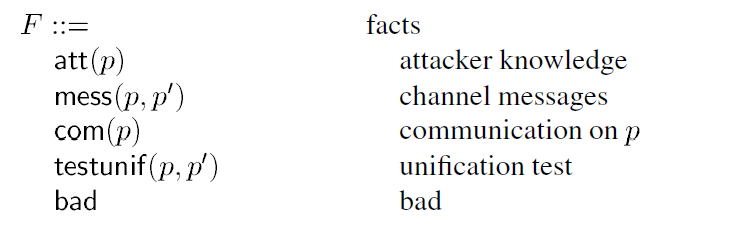
\includegraphics[scale=0.7]{Relazione/Immagini/fatti.PNG}
\end{figure}\\
Il fatto $att(p)$ significa che l'avversario può conoscere il valore di $p$. Il fatto $mess(p,p')$ sta a significare che il messaggio $p'$ può comparire sul canale $p$. Il fatto $com(p)$ sta a significare che l'avversario può comunicare sul canale $p$, il che permette ad esso di verificare che $p$ sia un nome oppure no. Il fatto $testunif(p,p')$ è definito come segue. Si dice che un insieme di pattern contengono nomi legati quando contengono sottotermini della forma $a[\dots]$ dove $a$ corrisponde ad una restrizione nel processo. Nella seguente definizione si utilizzano $Secr$ e $\sigma_0$ come nella Proposizione 1.\\
\\
\textbf{Definizione 3:} Siano $p,p'$ pattern chiusi. Si dice che $testunif(p,p')$ è vero se e solo se esiste una sostituzione chiusa $\sigma$ di dominio $Secr\ \cup \ EVar $ tale che $\sigma Secr$ non contiene nomi legati e $\sigma p = \sigma p'$, e non esiste una sostituzione $\sigma'$ di dominio $EVar$ tale che $\sigma' p = \sigma' p'$.
\section*{Esempi}
% Mostra gli esempi dell'articolo attraverso proverif
\end{document}